\documentclass[onecolumn, draftclsnofoot,10pt, compsoc]{IEEEtran}
\hbadness=1000 % suppress warnings
\usepackage{graphicx}
\usepackage{url}
\usepackage{setspace}
\usepackage{hyperref}
\usepackage{listings}
\usepackage{cite}
\usepackage{geometry}
\usepackage{pdfpages}
\usepackage{longtable}
\include{pygments.tex}

\geometry{textheight=9.5in, textwidth=7in}

% 1. Fill in these details
\def \CapstoneTeamName{		Aerolyzer}
\def \CapstoneTeamNumber{		19}
\def \GroupMemberOne{			Daniel Ross}
\def \GroupMemberTwo{			Logan Wingard}
\def \CapstoneProjectName{		Aerolyzer}
\def \CapstoneSponsorPerson{		Kim Whitehall}


% 2. Uncomment the appropriate line below so that the document type works
\def \DocType{		%Problem Statement
	%Requirements Document
	%Technology Review
	%Design Document
	%Progress Report
	Final Report
}

\newcommand{\NameSigPair}[1]{\par
	\makebox[2.75in][r]{#1} \hfil 	\makebox[3.25in]{\makebox[2.25in]{\hrulefill} \hfill		\makebox[.75in]{\hrulefill}}
	\par\vspace{-12pt} \textit{\tiny\noindent
		\makebox[2.75in]{} \hfil		\makebox[3.25in]{\makebox[2.25in][r]{Signature} \hfill	\makebox[.75in][r]{Date}}}}
% 3. If the document is not to be signed, uncomment the RENEWcommand below
\renewcommand{\NameSigPair}[1]{#1}

%%%%%%%%%%%%%%%%%%%%%%%%%%%%%%%%%%%%%%%
\graphicspath{{images/}}
\begin{document}
	\begin{titlepage}
		\pagenumbering{gobble}
		\begin{singlespace}
			\centering
			
\includegraphics[height=4cm,natwidth=345,natheight=435]{images/coe_v_spot1.png}
			\hfill 
			% 4. If you have a logo, use this includegraphics command to put it on the coversheet.
			%\includegraphics[height=4cm]{CompanyLogo}   
			\par\vspace{.2in}
			\centering
			\scshape{
				\huge CS Capstone \DocType \par
				{\large\today}\par
				\vspace{.5in}
				\textbf{\Huge\CapstoneProjectName}\par
				\vfill
				{\large Prepared for}\par
				{\Large\NameSigPair{\CapstoneSponsorPerson}\par}
				{\large Prepared by }\par
				Group\CapstoneTeamNumber\par
				% 5. comment out the line below this one if you do not wish to name your team
				\CapstoneTeamName\par 
				\vspace{5pt}
				{\large
					\NameSigPair{\GroupMemberOne}\par
					\NameSigPair{\GroupMemberTwo}\par
				}
				\vspace{20pt}
			}
			\begin{abstract}  
				The Aerolyzer Project aims to deliver a new source of air quality and weather information through leveraging existing weather data and image analysis algorithms.
				When complete, this open-source project shall feature a Python library that uses image classification and third-party weather APIs, displayed with an intuitive web-based user interface.
			\end{abstract}     
		\end{singlespace}
	\end{titlepage}

\tableofcontents
\clearpage

\begin{singlespace}

	\section{Introduction}
		Aerolyzer is a project initially proposed by NASA JPL that aims to deliver a new source of air quality and weather information through leveraging existing weather data and image analysis algorithms.
		Though lots had come up on the client's side of the project, and the details are a bit unclear, the client as of the end of the project is Kim Whitehall.
		The posible uses of the Aerolyzer python library include checking weather data to gain aerosol information in order to conclude whether alergy medication may be necessary.
		The project group initially consisted of three members, those members being Logan Wingard, Daniel Ross, and Kin-Ho Lam, though the project group finished with only two, those being Daniel and Logan.
		Kin-Ho Lam's name will be in the previous documents, though was not a part of the project as of winter term.
		Kim Whitehall was in charge of directing and managing the direction the project was going, while Logan and Daniel determined methods problems would be solved, as well as coding and implemeting these solutions.
		
	\section{Requirements Document}
		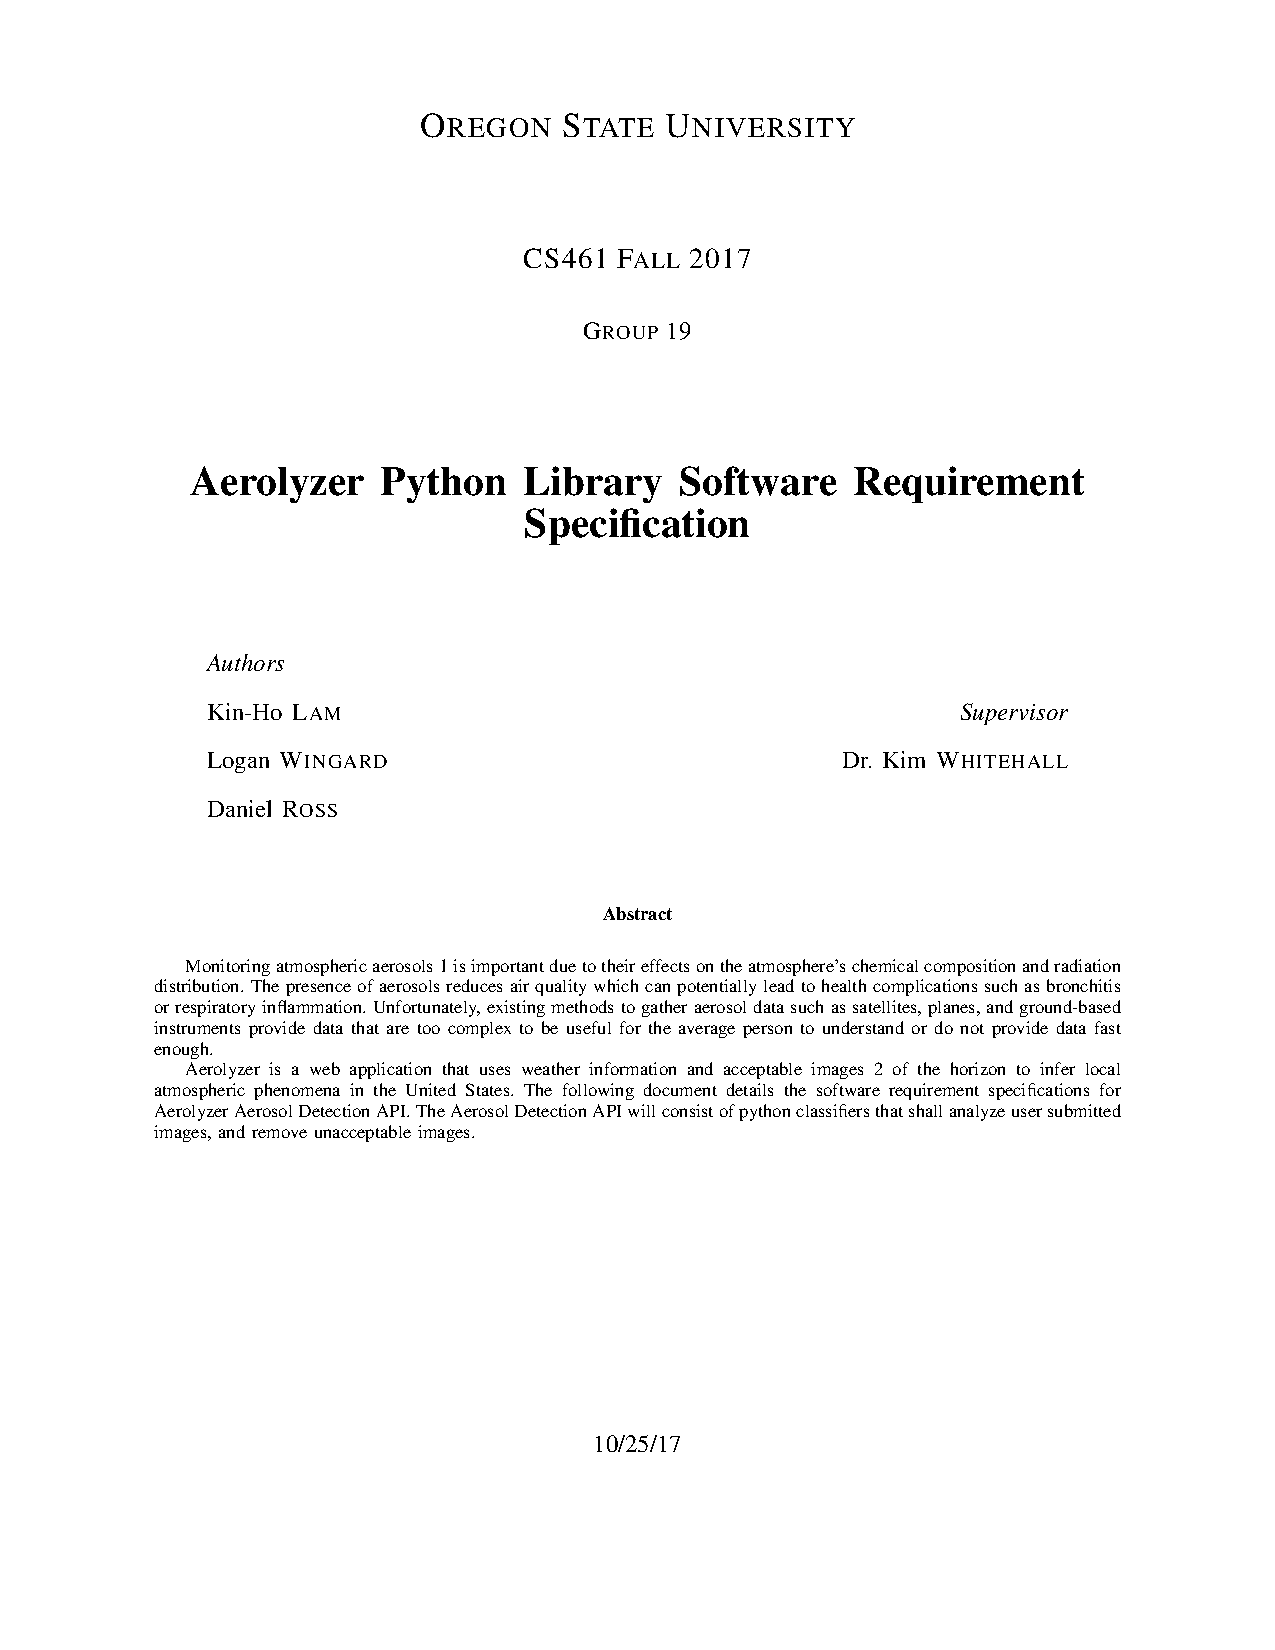
\includepdf[pages=-]{pdfs/require.pdf}
		The requirements for the project changed during winter term to better reflect what the client wanted and what the team would be capable of.
		The key difference is that the project focuses solely on the development of the Aerolyzer Python library rather than the creation of the library and the integration into the web application.
		Classifying the photo was simplyfied to be based solely on the horizon and the colors in the Haze Layer.
		Calling the Weather API was used to determine the time of Sunrise and Sunset in the test image.
		The Web Application interface was removed from the project.
		The Web application portion of ZIP Code Submission was removed, but the library instead uses an image's location data to determine ZIP code.
		Displaying the data on the Web Application was removed and a python graphing script was used to display the results of Aerosol analysis instead.
		
		
		In addition to these shifts away from the Web Application, our client expected the extraction and usage of image EXIF data be more extentensive than previously stated.
		Now handling the image EXIF data was expected to determine whether an image was taken during sunrise or sunset, rather than having an image classifier determine this.
		
		
		The reason behind many of these changes was the client's desire's being better accommodated and the loss of a team member making the integration of the library into a fully functioning application less feasible given time contraints.
		\begin{landscape}
			\subsection{Final Development Schedule}
			\begin{figure}[h]
				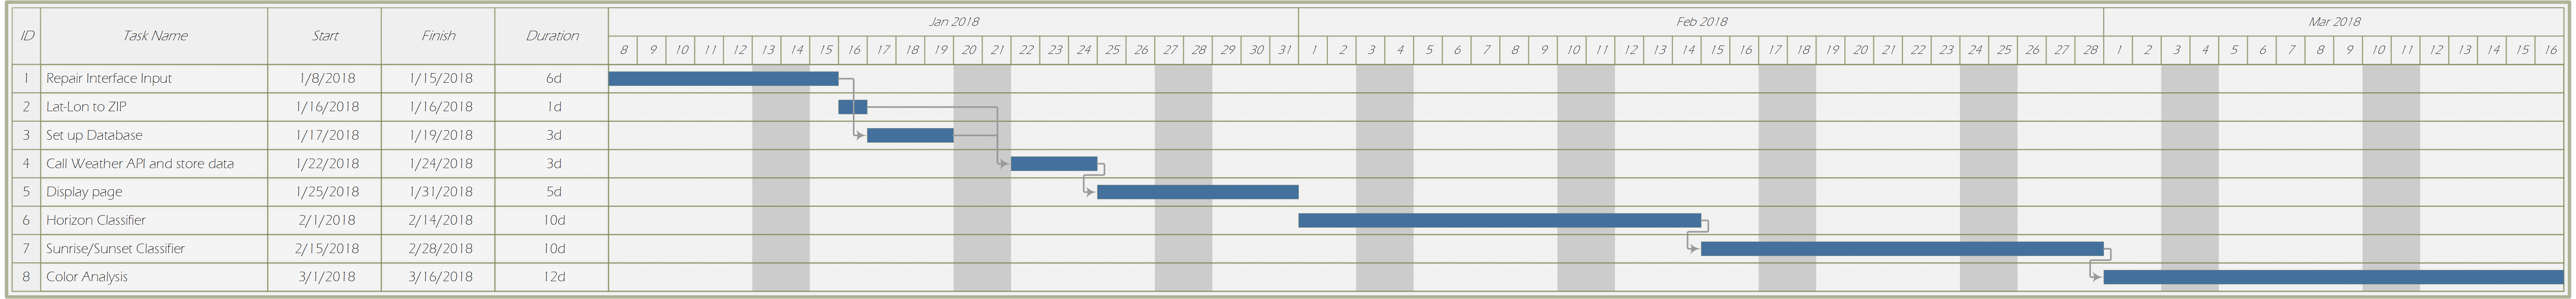
\includegraphics[width=9.5in]{gantt.png}
				\caption{Final Gantt Chart Schedule}
				\label{fig:Final Schedule}
			\end{figure}
		\end{landscape}
	\section{Design Document}
		The design document had been updated in Winter term as there were many design choices that we found to be impractical such as storing all the data to the database. 
		However, the most recent design doc that got signed is included below with more realistic design choices for horizon detection, color analysis and library structure.
		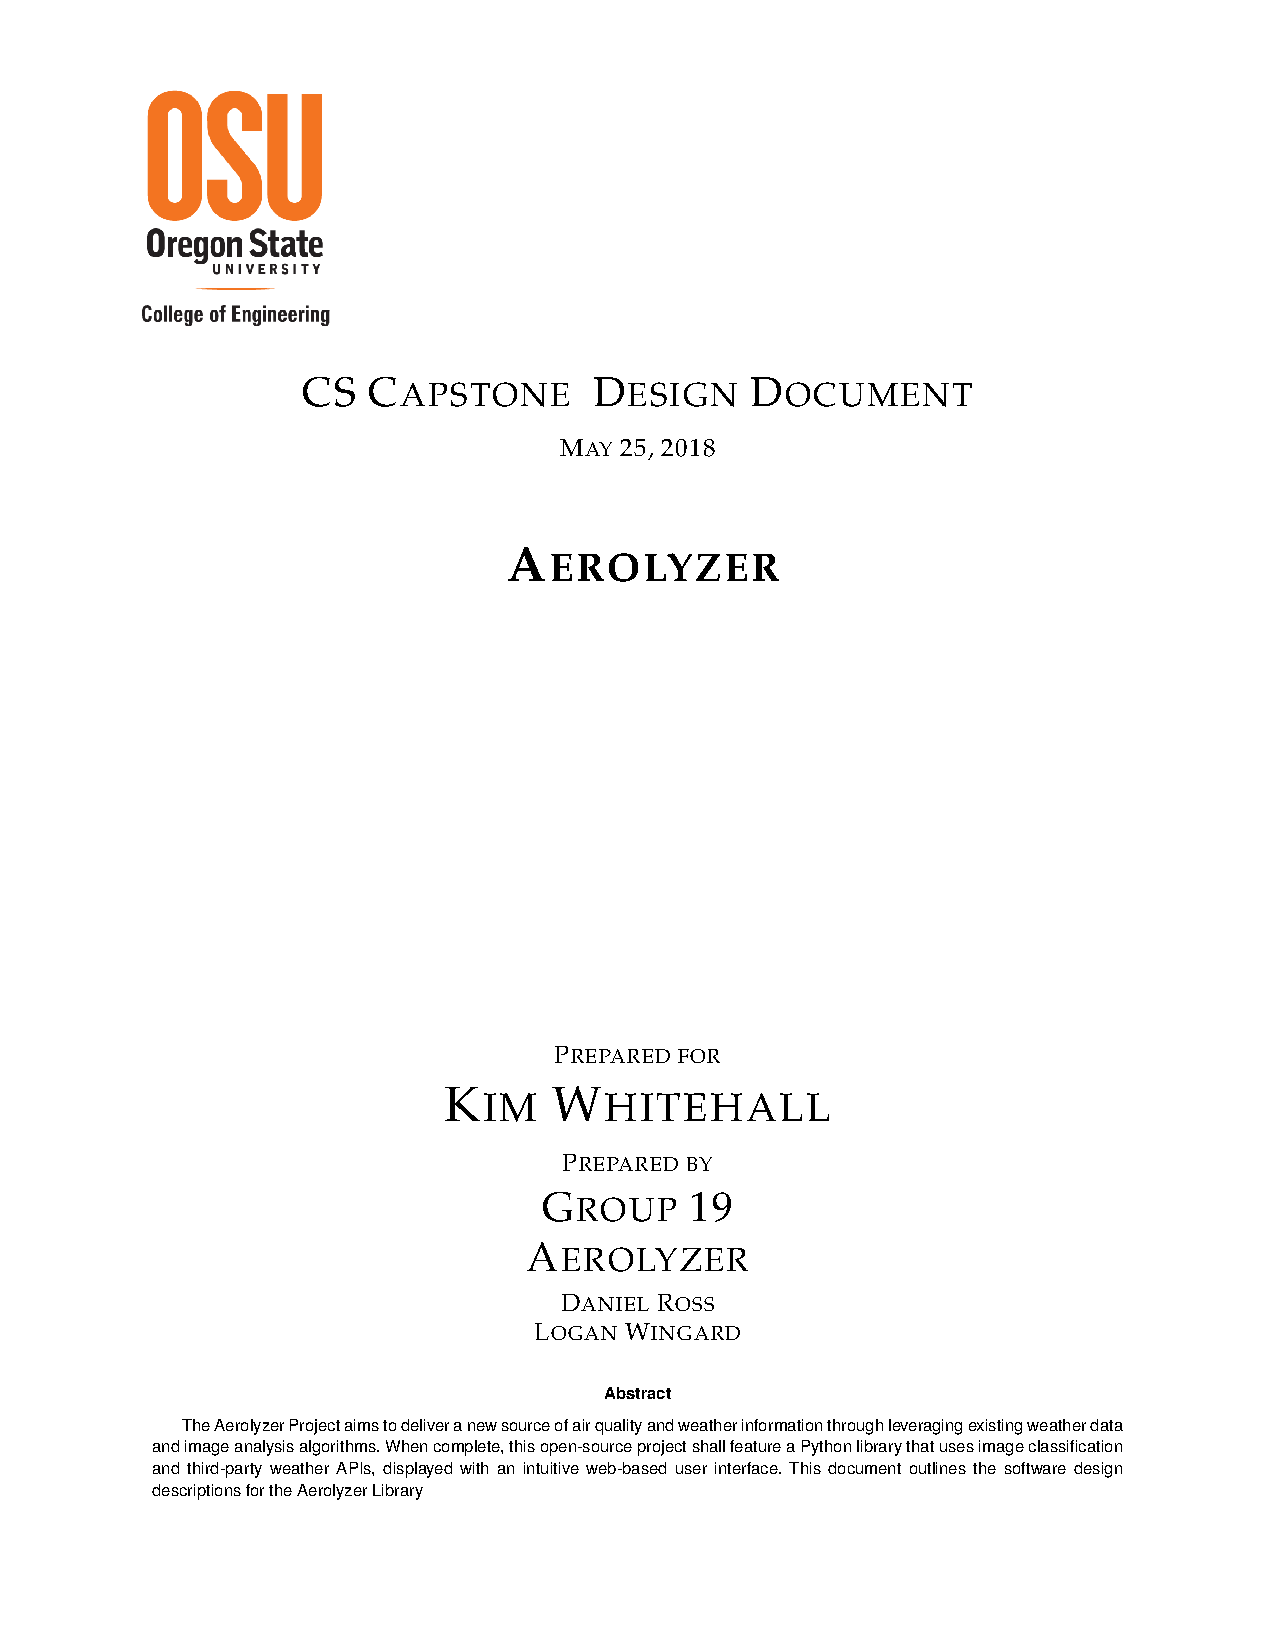
\includepdf[pages=-]{pdfs/design.pdf}
	\section{Tech Review}
		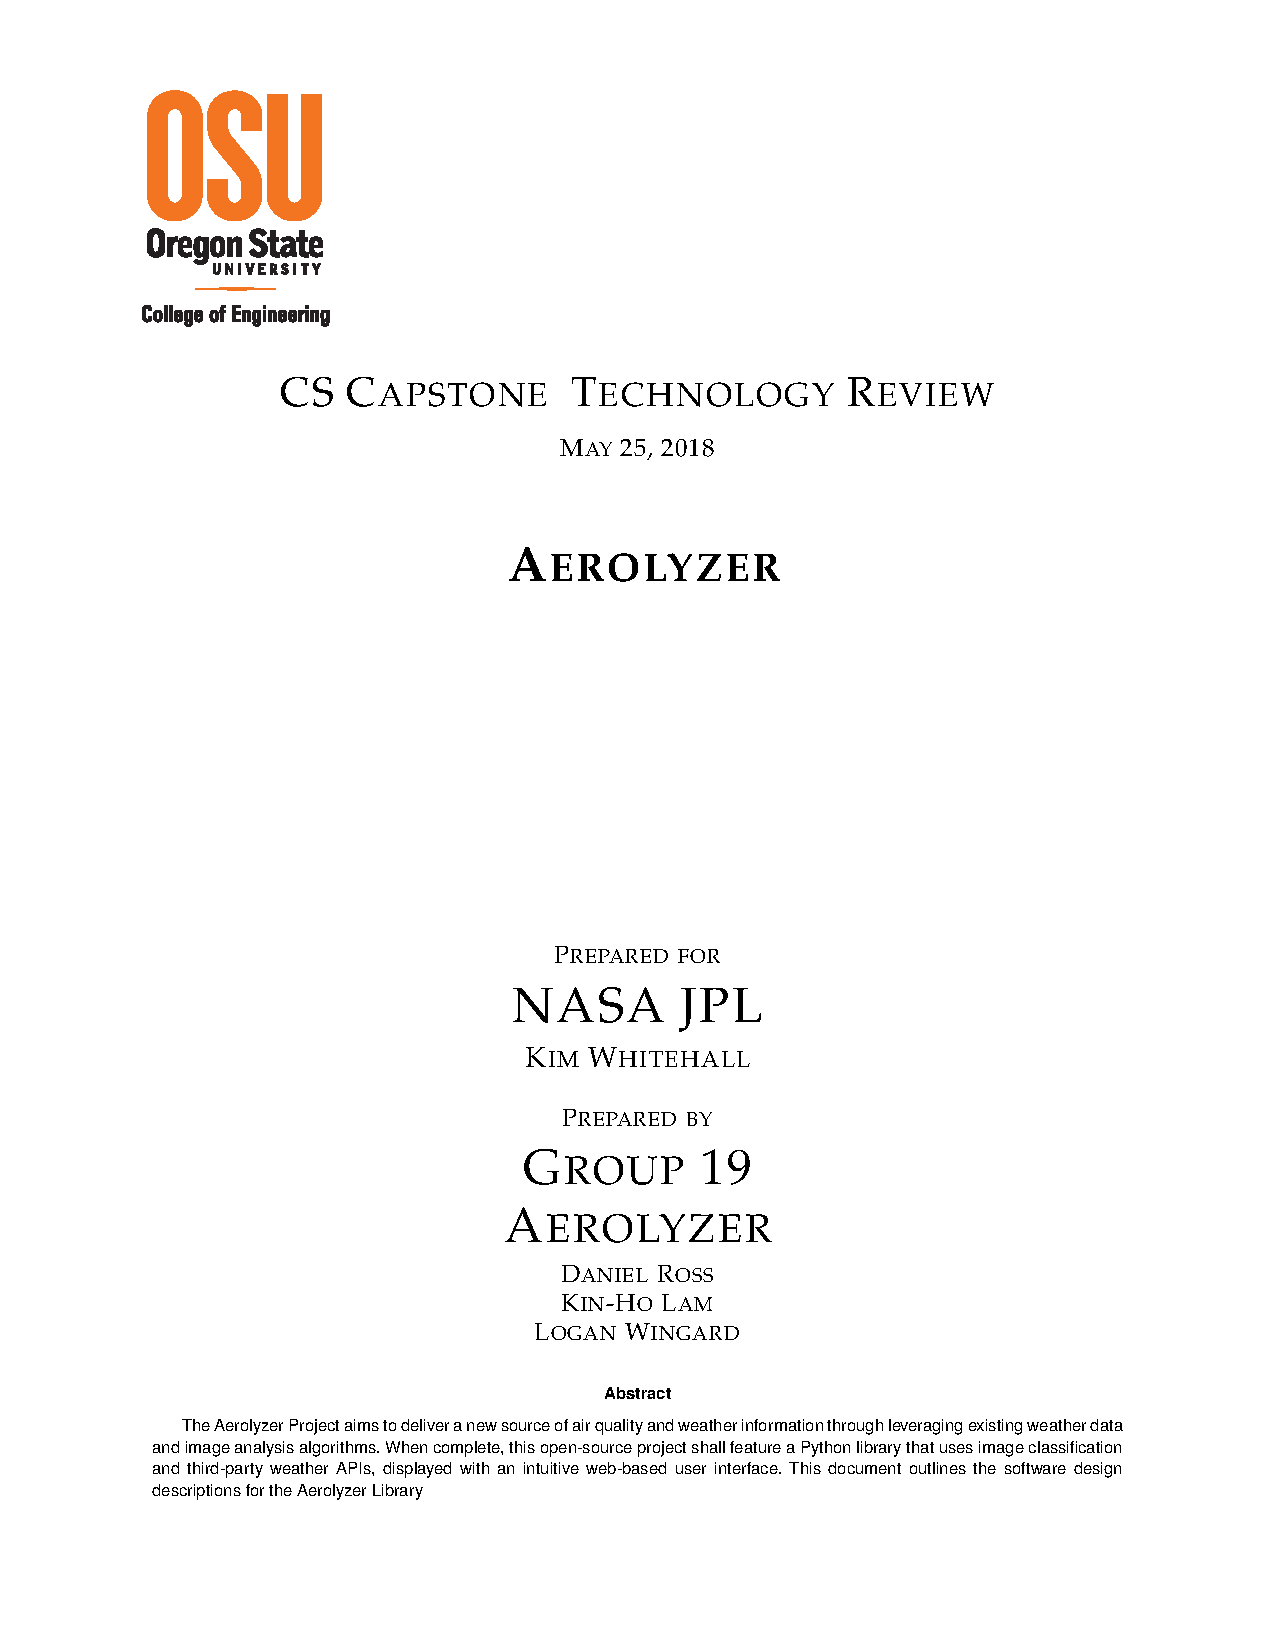
\includepdf[pages=-]{pdfs/tech.pdf}
	\section{Blog Posts}
		\subsection{Daniel Ross}
			\begin{longtable}{|l|p{0.3\linewidth}|p{0.3\linewidth}|p{0.3\linewidth}|}\hline \textbf{Week} & \textbf{Fall} & \textbf{Winter} & \textbf{Spring}\\\hline
			1 
			& I read the descriptions of all the projects.
			After reviewing them I decided on my top 5 potential projects.
			Only a couple of the possible projects actually scared me with their potential difficulty, but I selected one of those projects anyway.
			& Our client, Kim Whitehall, expressed that she was concerned with the direction that our team was going with the project.
			We had thought that we were on the right track, but this was discouraging.
			I was unhappy with how the meeting went and it felt like this was going to be an insurmountable problem.
			I planned on having our team rethink the entire approach to handling horizon detection, because machine learning seemed to be a time consuming rabbit hole without sufficient payoff.
			& We met with Kim and discussed that we need to add the code that we've completed on the virtual machines needs to be added to the github repository.
			I cleaned up my git commits and made my Wavelength functions into a pull request to add to the repo.
			I already have some code done for aerosol analysis, so I opened an issue for that specifically as Kim requested.
			I'm going to be going over my code to make sure it's ready to add to the main repository.
			\\\hline
			2 
			&I was assigned to the Aerolyzer project and met with my team before reaching out to our client.
			On Friday, our team met with our client, Dr. Whitehall, on a WebEx video conference.
			I need to research the pre-existing content in the project and gather an understanding of what our team will be adding.
			I'm researching the science behind aerosols in addition to reading the resources provided to us by Dr.Whitehall
			&The team met with the course professors to ask for advice on what the best course of action would be.
			Their advice helped convince me that changing the group's focus would be sufficient to succeed.
			Logan asked if I would meet with ombuds and him to discuss some issues with Kin-Ho.
			I attended that meeting hoping to come out feeling better about the team, but listening to Logan's concern made my opinion of how things were going seem more valid.
			Logan set up a meeting with Kevin and Kirsten regarding the group issues.
			& I went back to the Aerolyzer Design Doc and updated the color analysis section to match what we had for our Beta demo.
			I finished up a draft of the Aerosol analysis for the Beta demo.
			\\\hline
			3 
			&I started work on the problem statment, which is helping me gather my thoughts on the project.
			I also realized that if we're going to use location a good categorization would be ZIP code. Converting latitude and longitude into ZIP codes should be simple to implement.
			We've got to isolate what the end goal for our team is going to be.
			The last portion of the problem statement will have to be close to what Dr.Whitehall will expect from us.
			&Kin-Ho was removed from our group.
			I was extremely apprehensive at first since I didn't want to ruin his capstone or cripple our own development.
			It's hard working with new people and taking on strangers as clients, but this was more stressful than simply working on coding a project.
			By the end of the week I had a sense of relief that I knew I wouldn't have had if I wanted him in the group.
			I think these group issues have delayed the development a little bit.
			I'll fix and finish the location functions.
			&I spoke to Billy Buffum about his project at Ninkasi Brewing.
			His team's data management for the brewery's data seems interesting.
			I was busy this week with getting used to the Parallel Programming class without Professor Bailey, and I didn't spend as much time debugging the inputs on my aerolyzer functions as I would've liked.
			\\\hline
			4 
			&Dr.Whitehall approved of the content of our problem statement rough draft.
			Our problem statement rough draft had multiple issues and when turning in the final draft we were unsure as to whether we needed hand written signatures or just email validation.
			We're going to edit the first draft of the problem statement. In the future when a team member has questions I'll encourage them to ask a professor or TA if I don't have a solution.
			&I finished location.py.
			The functions can now pinpoint where a picture was taken down to the apartment.
			The Sun\_position function now returns whether an image was taken during sunrise, sunset, day, or night.
			The time ranges for sunrise and sunset may need to be adjusted.
			I need to figure out the simplest way to convert from a pixel to a wavelength.
			I plan on asking Kim in our next meeting for advice on these two issues.
			& Billy Buffum and I conducted our interviews for the Wired review articles and his project seems really useful for Ninkasi.
			For the Wired article I recreated the website's CSS and HTML formatting in my own review of the Ninkasi data management project.
			I restructured the functions in the aerolyzer library so that the main aerosol analysis is a class that can be called in the web framework and the other functions are just called by that class or the Image Restriction class.
			I installed PyLint on my virtual machine and figured out how to use it on specific files with the aerolyzer lint configuration.
			Kim asked me to lint the Wavelength Function commits made in the pull requests.
			\\\hline
			5 
			& Our team got around to experimenting on the Virtual Machine and testing OpenCv.
			Working on the requirements document has been tricky because my team is having difficulties with distinguishing design elements from requirements.
			Going forward in our requirements document we're going to remind ourselves that this paper is meant to describe the 'what' of our project. 
			&I've developed a first draft of wavelength.py which will convert from pixels to wavelengths.
			Kim wasn't available during our appointed schedule, but we still updated her via email.
			I'm not sure why but wavelength.py is varying wildly in accuracy.
			Ask TA for potential advice on improving accuracy.
			&I finished linting most of my code in time for our scheduled weekly meeting with Kim, but she didn't show up.
			Logan emailed her asking about her absence and hopefully we'll be able to get into contact with her soon.
			I'm feeling good about everything that's done on my virtual machine, but without Kim being available to review the code that gets added to the repo I'm a little concerned with what will be properly uploaded by the time Expo comes around.
			\\\hline
			6 
			&I started looking into how Google Tensorflow works. It may be a valid option for our horizon classifier.
			Tensorflow would be used as a supervised classifier which would require a large amount of pictures approved by our team. 
			I've started reading the Instagram API to see if there is an effective method for accessing images of the horizon in bulk.
			& During our meeting with Kim, I cleared up the time ranges for sunrise and sunset in sun\_position.
			Our TA, Daniel, told me that the accuracy of my method used in wavelength.py is dependent on the accuracy of OpenCV and the reference image.
			He also said that I should think of an alternative method if this one doesn't work.
			I'm going to try fixing this wavelength method, but if it's unsuccessful I'm going to scrap it and restart wavelength.py.
			& Logan and I finished up the midterm progress report and presentation.
			It feels like we haven't added much this term, but instead we've just ensured what we had works better together.
			We spoke with Kim again and my pull request for the Wavelength Functions was added to the repository at last.
			Now I can lint the Aerosol analysis class pull request and we'll be expo ready.
			\\\hline
			7 
			&I chose Development Environment, visuals for displaying our results, and database system as my research topics for my tech review.
			I've learned a bit about Docker conceptually, but still don't fully grasp how it's implemented
			I plan on downloading and experimenting with Docker to see if it will be a valuable tool for our team.
			& During our meeting with Kim, she pointed out that the image I was using for my comparison array had values that compensated for what human eyes can see. The next day I found a program, Spectra, which converts from wavelength to RGB that also puts out a visible light spectrum. After replacing the reference image with the new image of the visible light spectrum the wavelength output was accurate.
			Now that I have the accurate wavelengths I need to figure out the best method to use them.
			I'm going to research the Rayleigh Scattering effect and the Mie Scattering effect.
			& Logan came to me a few days before expo and pointed out a few bugs concerning the scope of some function calls within the library.
			After we sorted those out we wrote a small script using the PyPlot library to show the aerosol analysis results in a bar graph.
			Using the small script to show the results of the library, we had a great expo.
			I felt well prepared for all of the questions we got at expo and despite my fears everything went well.
			\\\hline
			8 
			&Kin-ho found an implementation of Tensorflow that was in a Docker container, so I set up a Docker for us and got some practice assembling containers.
			At the end of the peer review I was aware that I had to replace my Development environment research with something else.
			I researched Web Frameworks, I chose this as a topic so that I'd better understand the work the previous Aerolyzer team accomplished.
			& There wasn't much progress this week as I'm struggling to find a way to connect the Rayleigh scattering effect to the size of aerosols.
			I plan on looking for some simple relationship to express the Rayleigh Scattering effect. It may just end up being a placeholder for a different relationship.
			&We had our last meeting with our client, Kim, and we got to tell her about expo.
			She asked about the script we wrote for the expo demonstration and we sent her a copy of it.
			Now that the bulk of the project is over I'm thinking about the Final Presentation and what we're going to record for it.
			\\\hline
			9 
			&When our team met with our TA and discussed our Requirements document, he pointed out some elements in the requirements document that would be better suited for the Design Document.
			Dr.Whitehall expressed frustration with the fact that she wasn’t fully in the loop on our test code not being on the github repo.
			Improve our team’s communication channels with Kim.  I plan on rereading the framework that the previous team left us to see if we’ll need to make any additions.
			&I found a chart of aerosol sizes that shows the range of sizes that the aerosols cover. Using these sizes I can create a target for the wavelength that's captured from the images.
			The process of converting from a pixel to a set of scores for the possible aerosols is too slow. I ran it on a test set of pixels and the average speed was about 0.004 seconds.
			Ask our TA and Kim for advice on speeding up the function.
			& Logan prepared a script for the Final Presentation and I reserved a room at the library so that we could record.
			I recorded a second part specifically about how the aerosol analysis works in the final project and then I edited the video.
			\\\hline
			10 
			&On Tuesday we called Kim and we talked over the expectation for github and further development for Aerolyzer. I feel like we’ve cleared everything thing up for now, but I’m going to have to remember to keep up with the open source development. 
			Our team spent hours trying to get the LaTex document formatting to work properly when we compile it.
			I plan on reading the long LaTex guide and seeing if there are any packages that could help us understand any errors we make. Ideally I will find a LaTex IDE that doesn't conflict with the LaTex resources on the OSU servers.
			&Logan's haze layer function is successfully producing samples that are then passed into my aerosol function. We trimmed the sample size to 1000 pixels so the process wouldn't take to long.
			Our TA told me that since our library is written in Python, we may have to live with the fact that the aerosol function is slow. He said to look for the point in the process that is the slowest and try to improve that, but since Python doesn't do multi-threading it may be difficult to speed up.
			I'll look for a way to optimize the function.
			&I was very busy working on final assignments for other courses, but I was relieved to see how much Logan had prepared for the final paper.
			Now all that I have to do is help where I can and try to finish this course strong.
			\\\hline
			
			\end{longtable}
		\subsection{Logan Wingard}
			\begin{longtable}{|l|p{0.3\linewidth}|p{0.3\linewidth}|p{0.3\linewidth}|}\hline \textbf{Week} & \textbf{Fall} & \textbf{Winter} & \textbf{Spring}\\\hline
			1 &
			Set up one note (I think) 
			Looked over projects. Very interested in the 3d vr painting project.
			Reached out to Mike Bailey & One Group member was removed for the group

Kim also mentioned that we were low priority with her new schedule. 
I take this more as a challenge to prove her wrong with some good code output & I have been working on linting, cleaning and testing my code.
I am planning on creating a pull request with these changes soon.
			\\\hline
			2 & 
			Assigned to team 19 Aerolyzer
			Met with client 
			We discussed goals, technicals, and made a plan for the problem statement  & Daniel has written a lon lat conversion function to get it in a more usable format

We need to start making database decisions, what needs to be saved on the database and what doesn't.

We are also informed that we need to remove NASA JPL from all docs, as there is no longer a connection between Aerolyzer and NASA. & Lots of bug testing this week. Through some tests, I found that my accuracy was short by a bit, so I improved my algorithm to rach the desired accuracy
			\\\hline
			3 & 
			Summary: 
			We had another meeting with our client, this one had a focus on project requirements.

			We also met with our TA for the first time :
			Narrow down requirements.
			Bring 3x5 notecard to write requirements down. If it doesn’t fit, narrow down.
			Nail down EXACTLY what client wants
			Don’t be afraid to negotiate with client. 
			Do something silly to familiarize with framework. & Worked a bit on image classification, only to realize most of them have already been completed by the previous group, without our client's or my knowledge.

Daniel has also made great progress on location functions. & We are starting our wired articles. They are basically "reviews" for eachother's projects.

I met with Dennie DeVito in class and we agreed to interview each other for the assignment.
			\\\hline
			4 & We were able to get the problem statement in.
We will look into what the requirements doc is. We've also been experimenting with the vm and opencv & Been working on my code for horizon detection. Still brainstorming about methods do do this. Right now I am able to single out the sky if one is present in an image. Still not very accurate & I emailed dennie again with no response. I contacted Kirsten to let her know about the situation and she informed me another classmate also had a similar issue, which works out great for the both of us. We interviewed each other and were able to write our articles and submit them on time
			\\\hline
			5 & We have a very good draft of the requirements doc. Our rough draft was missing a Ghant chart, though I'm fairly happy with the draft. & I'm having a lot of issues with git. My algorithm for horizon detection is covered over about 30 commits and that is too much to look over for one pull request. Worked on rebasing and linting code to make both the code and the pull request more readable & For an unknown reason, Kim has not been replying to emails. Last meeting, she mentioned that she was not feeling well, so we are hoping eveerything is alright. 

The issue with the config files has hopefully been resolved. When we regain contact with Kim, we will show her our methods and hopefully get some direction. 
			\\\hline
			6 & 
The final requirements doc looks really good. Got a very good looking ghant chart. 
We have still been looking into importing python libraries and how to create one. 
We also found some code that shares many of the functions that we hope to use. We plan on contacting the creator and ask permission. There also has to be edits to the code to actually make it usable, considering the code we found takes in live video while we only need to use it for 1 picture at a time. 
& I've decided to try to implement some machine learning into my horizon detection as I am unable to make the 66\% accuracy goal. Been messing arround with neural networks and I'll see where that leads
 & Kim reconnected with us after a couple weeks of silence and we were able to get back on track.

With her guidance, we decided to combine our two fixes to the config issue and we now have a working library that is ready (hopefully) for expo
			\\\hline
			7 & After looking more into python modules, I was able to get the module set up correctly.
We ended up not using the horizon code that we found because it wasn't very compatible. We are going to try to write one from scratch. & Continued working on Neural network for horizon detection and it reached the 66\% benchmark. That is about all I've been able to work on over the week & When testing our library for expo, I found sevevral bugs that luckily had simple fixes. I have opened a github issue ad I will create a pull request fixing these bugs sometime after expo.

Expo went really well. If anything, we overprepared, going as far as to bring a whiteboard for explanations to really technical questions that were (thankfully) never asked.
			\\\hline
			8 & I messed up when pushing to github and our client is not a happy camper. 
I agreed to have a 1 on 1 with our client to discuss git workflow.  & Cleaning up and linting code before I make a pull request. I'm moving onto color extraction and getting the data from the haze layer to the functions that Daniel has been working on for color analysis & Post expo, it is now time to start working on final documentation. Start getting all the git issues and weekly blogs together for the report, and start putting a script together for our final presentation.
Lastly we will need to fill out peer reviews and sign off the code to our client.
			\\\hline
			9 &  Had a good break. Set a time for meeting with client.  & Color extraction was pretty simble as the code I used to find the horizon was very helpful in singling out the haze layer.  Made it so it will chose 1000 random points to pass to the color analysis. & Not much left to do except keep working on documentation. the code has been completed.
			\\\hline
			10 & We've been working on the design doc. Trying to get that submitted on our team one note. Looks like we won't be able to start our progress reports until the weekend.  & The only thing I'm really able to work on this week has been the progress report. Will get that writen up, recorded and submitted & We finished and submitted our final presentation, all that is left to do is finish with this report.
			\\\hline
			
			\end{longtable}
	\section{Poster}
		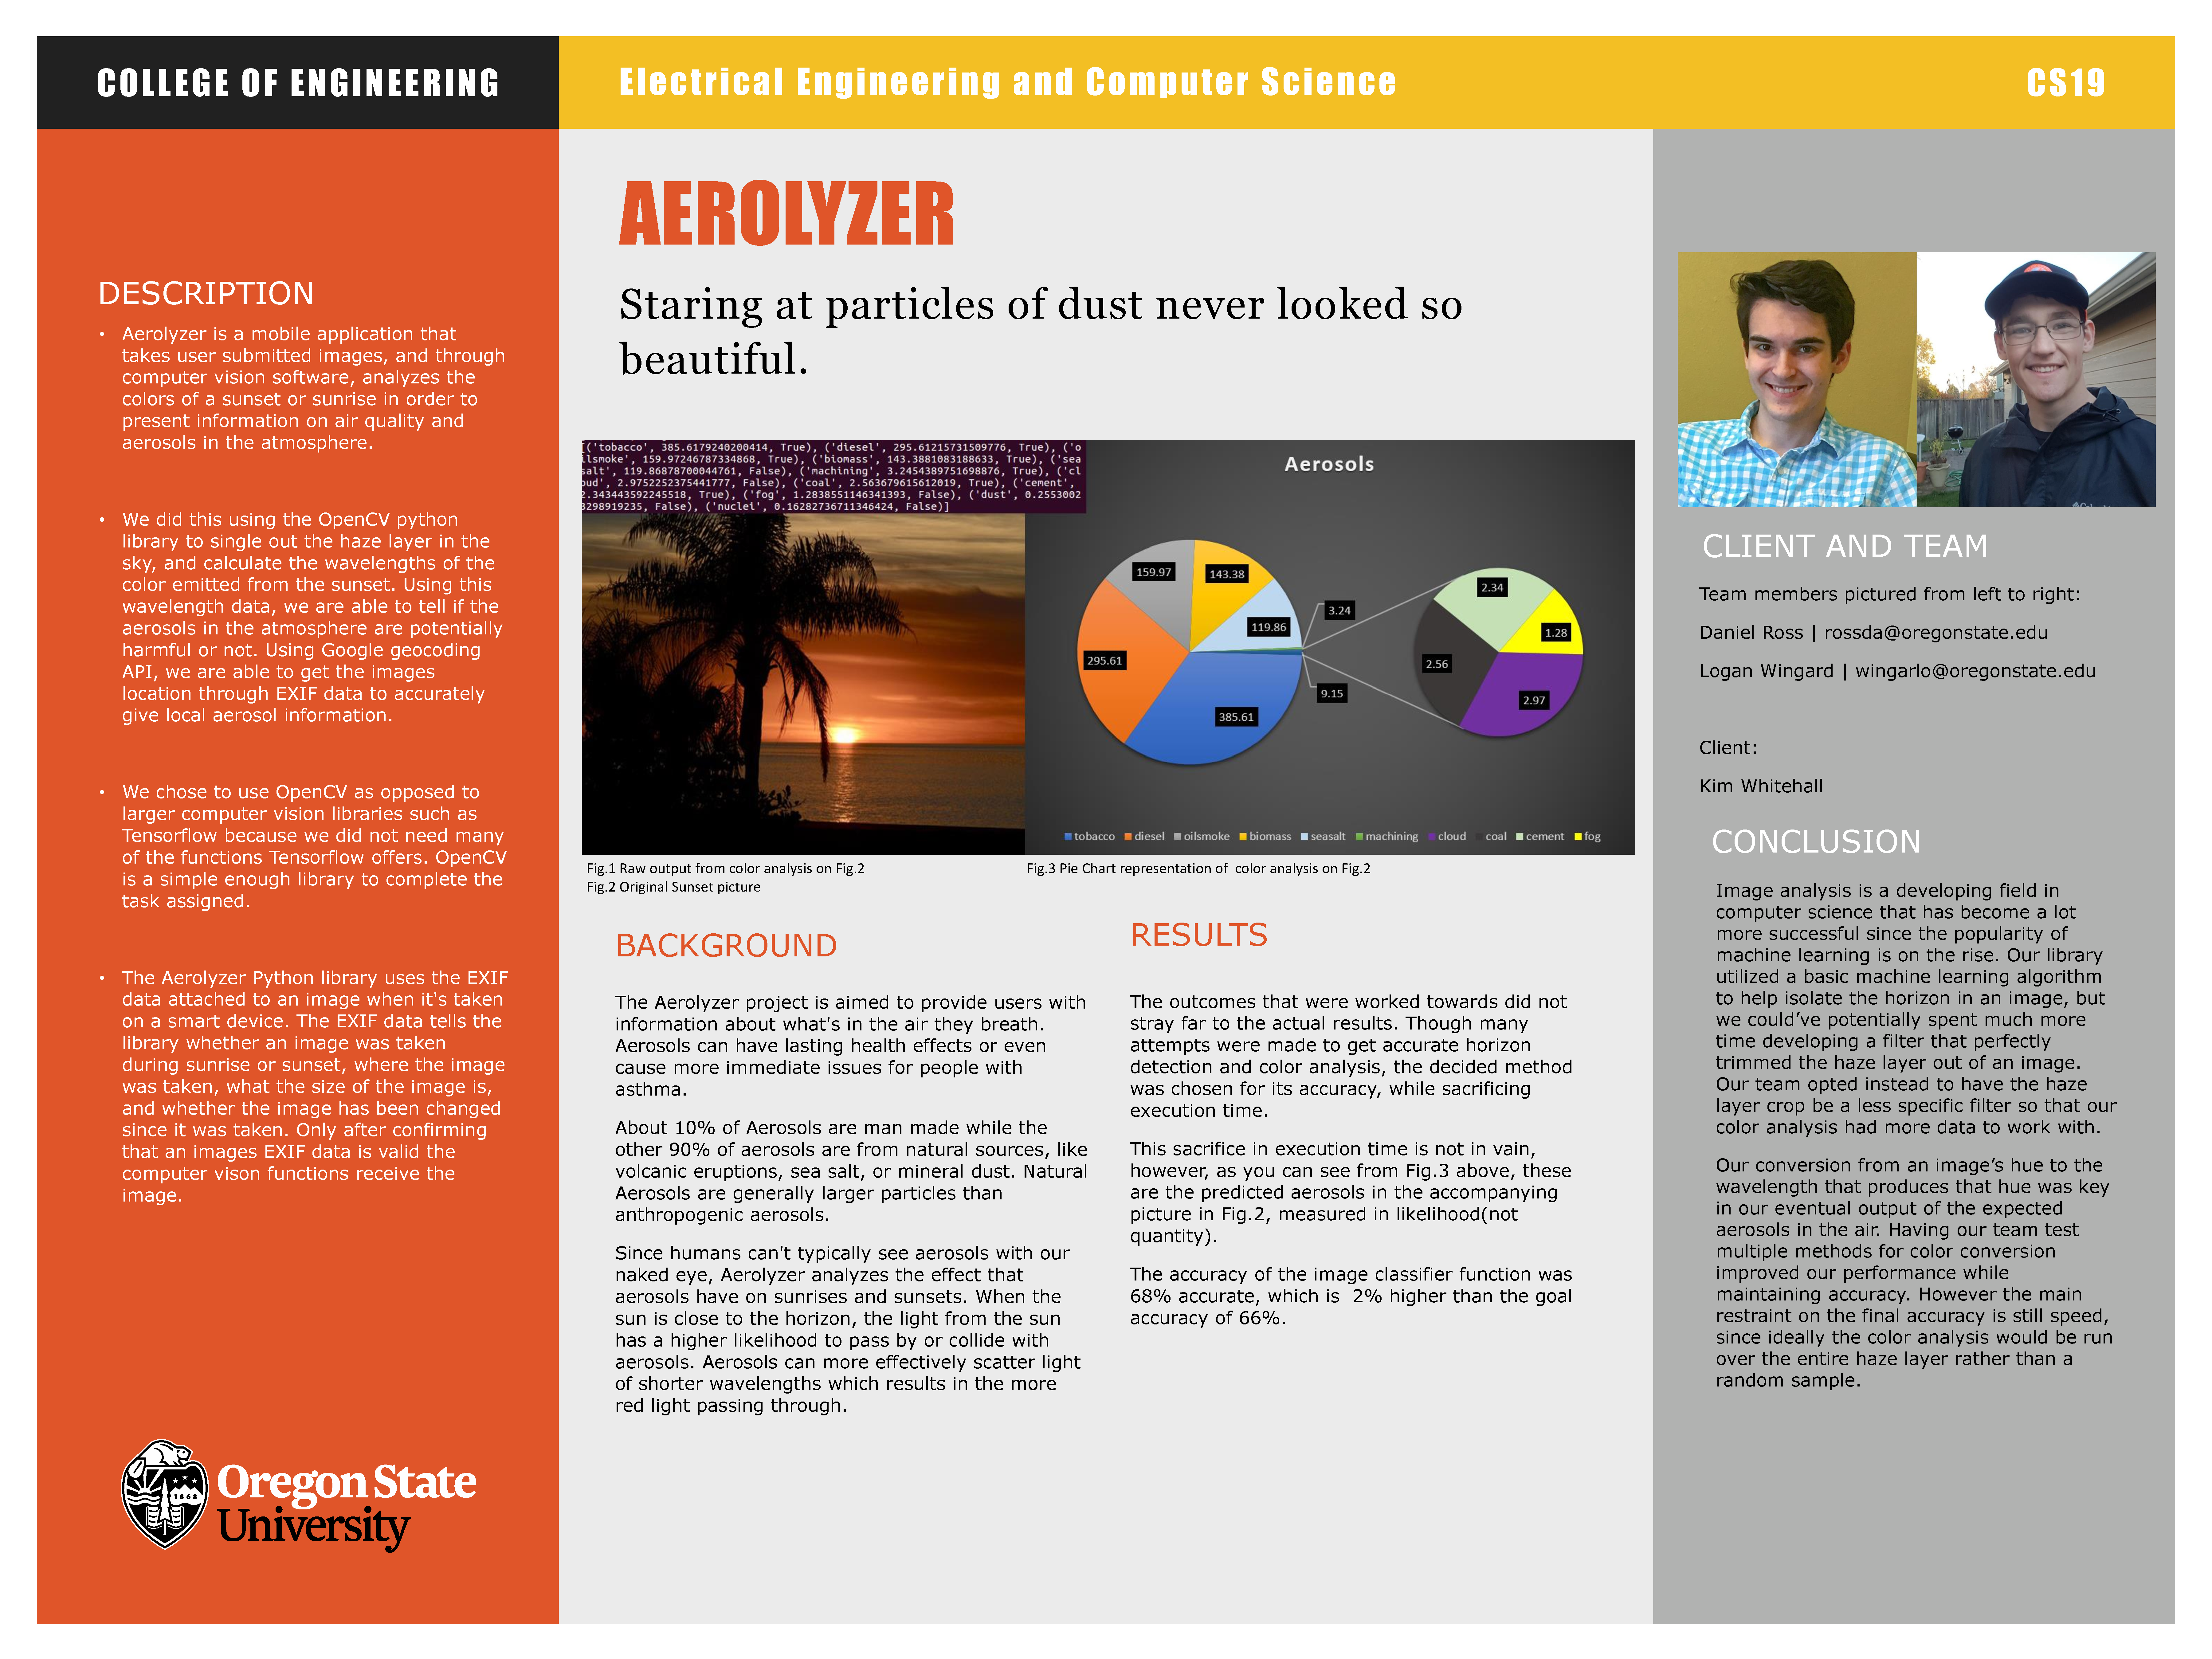
\includepdf[pages=-]{pdfs/poster.pdf}
	\section{Project Documentations}
		Documentation on the code can be found on the Aerolyzer Github.
		To preserve the format of the issues and Pull requests, follow the links below to view them as intended.
		\url{https://github.com/Aerolyzer/Aerolyzer/issues}
		\url{https://github.com/Aerolyzer/Aerolyzer/pulls?q=is%3Apr+is%3Aclosed}
		
		Aerolyzer is completely open source, meaning users are able to install the python package directly from Pypi.
		After installing Aerolyzer using pip install aerolyzer, and ensuring you have all of the requirements that should automatically install when installing aerolyzer, you now have access to the Aerolyzer library.
		The three classes that are included in this library are imgRestFuncs, RtrvData, and AeroData.
		
		With these objects created, you are able to classify images using imgRestFuncs, retrieve the image's data using RtrvData, or detect aerosols using AeroData.
		There will be a script included in the code submission named expo\_demo that will make a use of these classes.
	\section{Recommended Resources for Learning More}
		Aerolyzer is completely open source and is even on the Python Package Index (pypi).
		To learn more about how Aerolyzer works, all the code and documentation is on the Aerolyzer github.
		Some of the resources used to learn the techniques implemented into the Aerolyzer library include the following.
		Neural networks:\\
		\url{https://github.com/llSourcell/Make_a_neural_network/blob/master/demo.py} \\
		\url{https://iamtrask.github.io/2015/07/12/basic-python-network/} \\

		Aerosols:\\
		\url{https://aeronet.gsfc.nasa.gov/new_web/Documents/Aerosol_Optical_Depth.pdf} \\

		Pypi:\\
		\url{https://packaging.python.org/tutorials/distributing-packages/#setup-py} \\
		
		Color information: \\
		\url{https://www.weather.gov/jetstream/color} \\
		\url{https://en.wikipedia.org/wiki/File:Linear_visible_spectrum.svg} \\
		\url{http://steve.hollasch.net/cgindex/color/freq-rgb.html} \\
		\url{http://www.efg2.com/Lab/ScienceAndEngineering/Spectra.html} \\
		\url{http://www.physics.sfasu.edu/astro/color/spectra.html} \\

		This is the code that was used to generate the image being used. \\
		\url{http://www.gringene.org/code/spectrum.r} \\


	\section{Conclusion}
		\subsection{Daniel Ross}

			Over the year I became a competent python programmmer.
			In addition to this I learned how to properly use public APIs and I relearned how to use git as version control.
			Unexpectedly I was also reaccquainted with optical physics and statistics.

			The expo and all of the preparation leading up to it reaffirmed how important interpersonal skills are in any field.
			I may only be working on a computer most days in my career, but that doesn't mean I shouldn't know how to carry a professional conversation.

			Having a well developed plan is very useful, but that doesn't mean that sticking to that plan is always correct.
			When our client said that things we're moving away from what she wanted, we had to adjust our plan and quickly move forward.


			Delegating certain tasks to certain team members is sometimes difficult when you don't know the exact difficultly of a task before it's underway, but the benefit of having the project split up into managable pieces outweighs that initial risk.
			Keeping up with version control is very nice for referencing purposes and makes the process of figuring out what's been complete easy.
			That said sometimes the overhead of version control can get in the way of progressing a project if the team isn't on top of it at all stages.

			Working in a team has been difficult for me in the past.
			While I can say it's still not easy, I have learned about the importance of clear communication.
			Taking a team member's input seriously is important, but I learned that if there's something you disagree with or don't understand you need to make it heard by the rest of the team.

			During the first term our team had trouble taking the client's input to heart and there was a lot of development time spent on an aspect of the project that ended up being one small part of the project as a whole.
			Personally my largest mistake during capstone was going along with this design idea rather than looking into other options that more closely matched what our client was asking for.
		\subsection{Logan Wingard}
			Coming into this project, I was very unexperienced when it came to git and maintaining a consistent version control.
			Now that we are finished, I can safely say my skills maintaining version control have increased greatly.
			I now feel as though I would be able to work on large projects in the future without having to hassle with git.
			
			Though python was one of my strongest languages coming in, it is by far my strongest language now.
			Through extensive practice using python classes, and using an array of python libraries, I am now able to do things with python I neve imagined.
			
			I won't lie, a lot of things went wrong in this project. 
			Most of these issues were due to poor communication.
			I have learned that things going wrong is not abnormal when it comes to projects, and after seeing the outcome of a project that went this poorly, I am excited to say I am prepared for the worst.
			
			Lastly, it was nice to get some information from a field other than computer science.
			I learned a lot about aerosols\cite{allen_2015} and their affects on the colors of the sky, as well on the affect on humans.
	\section{Appendix}
		Here is a script that should help testing the library.
		You may notice a path \/images\/test2.jpg.
		You would need to replace that with your image's location.
		It also requires the import of a package called plotly.
		\begin{lstlisting}
import os
import aerosol
from image_restriction_main import check_image
import sys
import plotly
import plotly.graph_objs as go
from image_restriction_functions import imgRestFuncs as Fxn
from retrieve_image_data import RtrvData as Data

if(check_image("./images/test2.jpg")):
	aero = aerosol.AeroData("./images/test2.jpg")
	x = []
	y = []
	colorIN = []
	results = aero.aerolyzeImage()
	for a,b,c in results:
		x.append(a)
		y.append(b)
	for TFval in results:
		if (TFval[2] == True):
			colorIN.append('rgba(215,63,9,1)')
		else:
			colorIN.append('rgba(0,0,0,1)')


	data = [go.Bar(
		x = x,
		y = y,
		marker=dict(color=colorIN)
	)]

	plotly.offline.plot(data, filename = "aeresults.html")

		\end{lstlisting}
		This script will also open up an html bar graph showing the results.
\end{singlespace}
\clearpage
\bibliographystyle{IEEEtran}
\bibliography{ref}
\end{document}
